\chapter{Effect of Operating Systems on Results}

\section{Overview}

\begin{table}[htb]
  \begin{center}
  \begin{tabular}{|l|c|c|>{\centering\arraybackslash}p{3.4cm}|} 
  \hline
  \textbf{Environment} & \textbf{Linux} & \textbf{Mac} & \textbf{Windows} \\
  \hline \hline
  Compiler & g++ 8.4.0 & Apple clang 11.0.0 & g++ 10.2.0 (Mingw-w64) \\ 
  Operating System & Ubuntu 18.04.05 & macOS 10.15.7 & Windows 10 Version 1809 \\ 
  % Kernel & GNU/Linux 4.15.0-117-generic x86\_64 & x86\_64-apple-darwin19.6.0 & WIN32 \\ 
  CPU & 0.3 & Intel Core i5-4260U & Intel Core i5-4670 \\
  Cores & 32 & 4 & 4 \\
  \hline
  \end{tabular}
  \end{center}
  \caption{OS Specifications}
  \label{tab:OSspecs}
\end{table}

\begin{figure}[htbp]
  \centering
  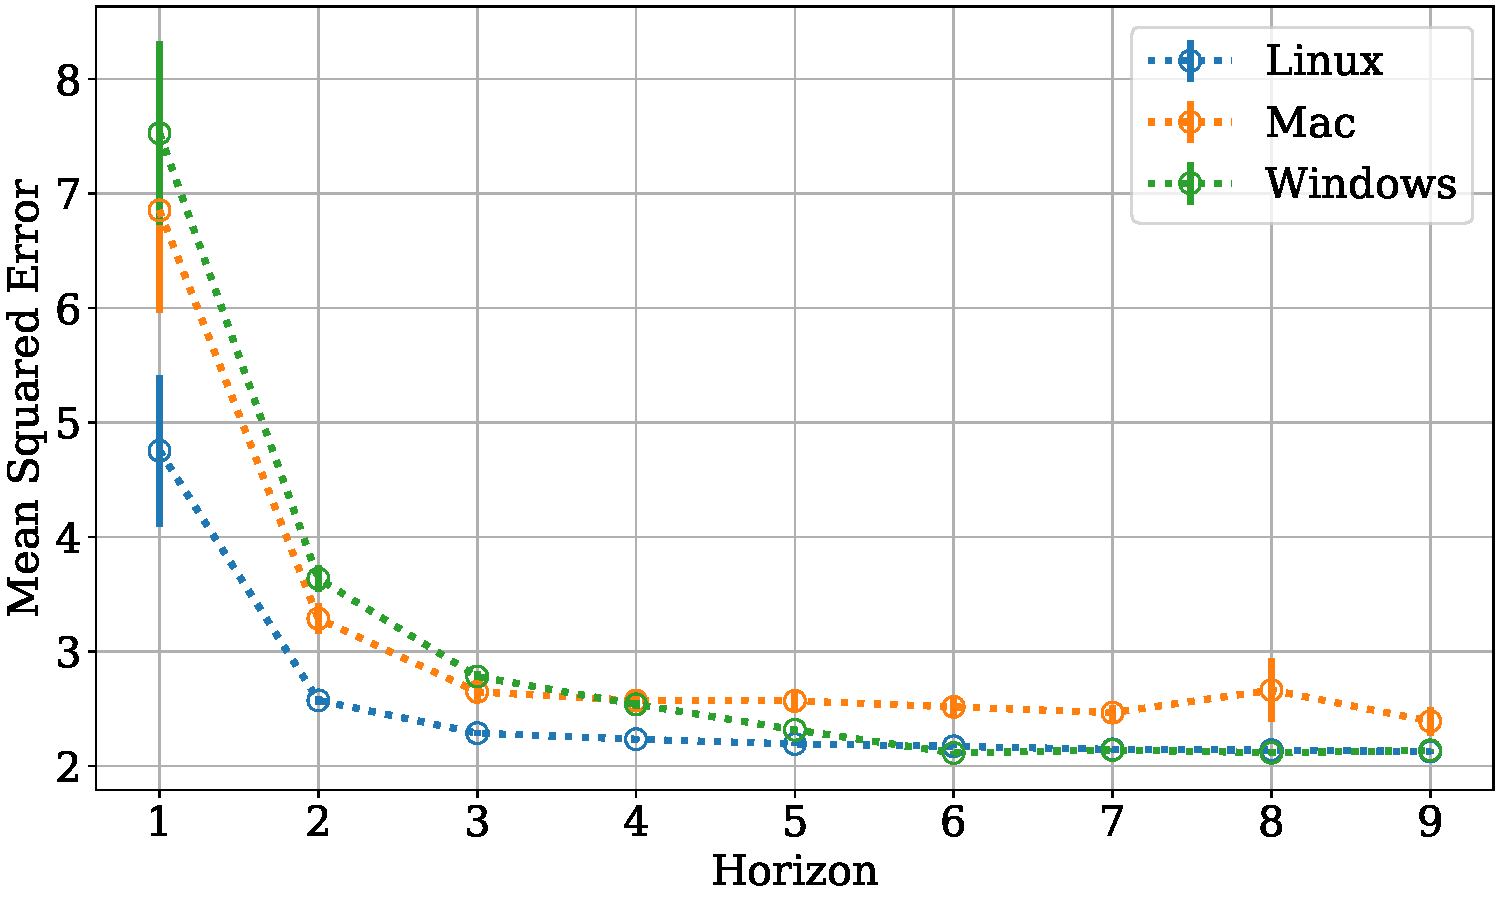
\includegraphics[width=0.8\textwidth]{OS_MSE_against_H} 
  \caption{Average MSE vs. finite Horizon $H$ on different OS}
  \label{fig:OSmse}
\end{figure}

\begin{figure}[htbp]
  \centering
  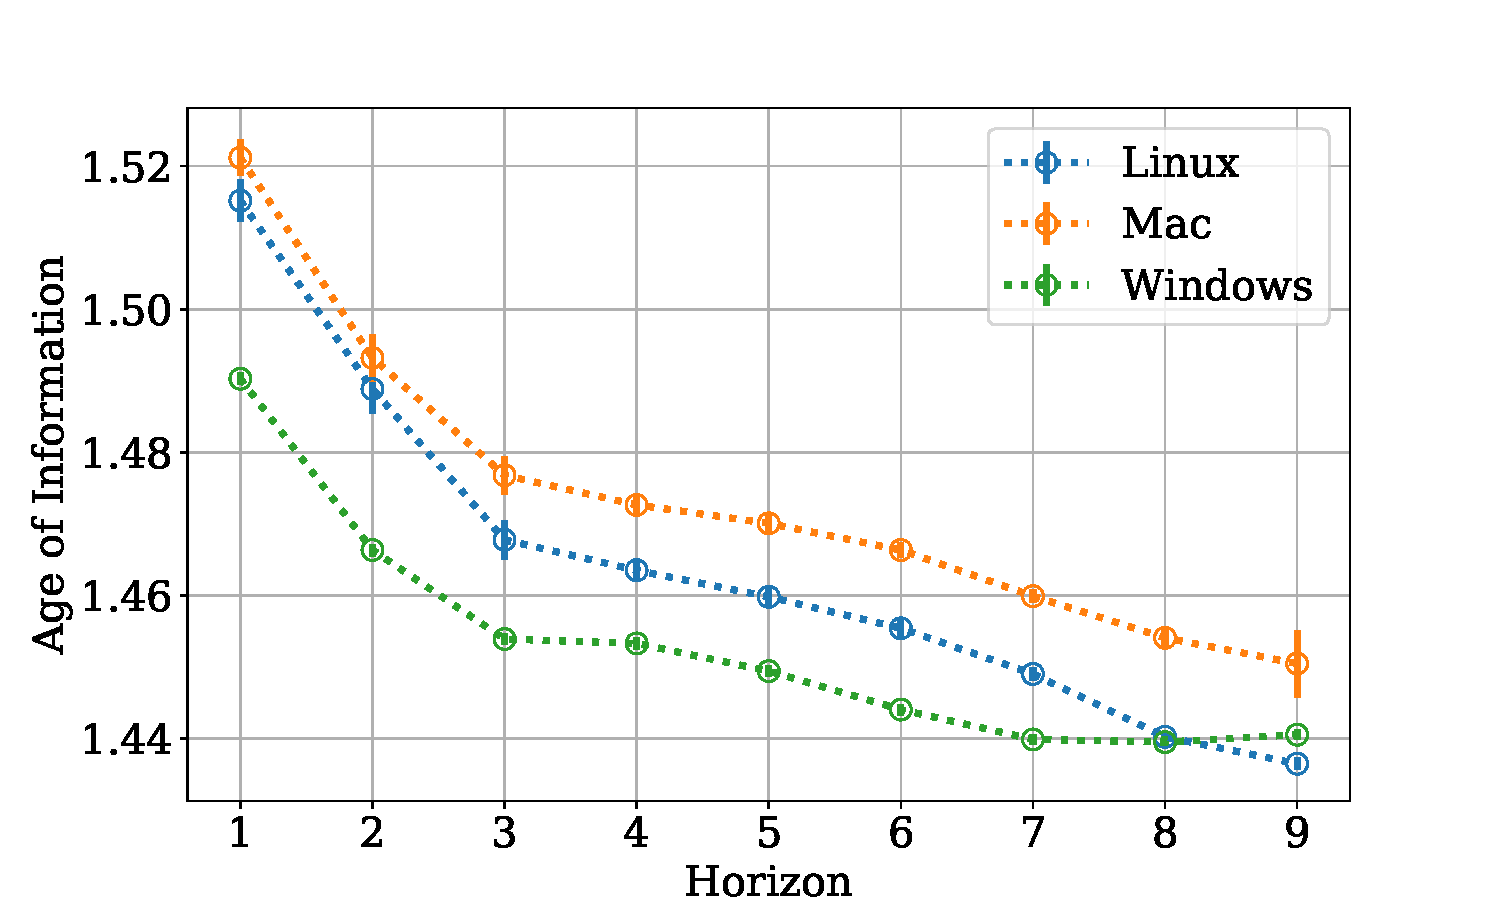
\includegraphics[width=0.8\textwidth]{OS_AoI_against_H} 
  \caption{Average AoI vs. finite Horizon $H$ on different OS}
  \label{fig:OSaoi}
\end{figure}

\section{Numerical Experimentation}

\subsection{Random Number Generator}

\begin{figure}[htbp]
  \centering
  \begin{subfigure}[b]{0.49\textwidth}
      \centering
      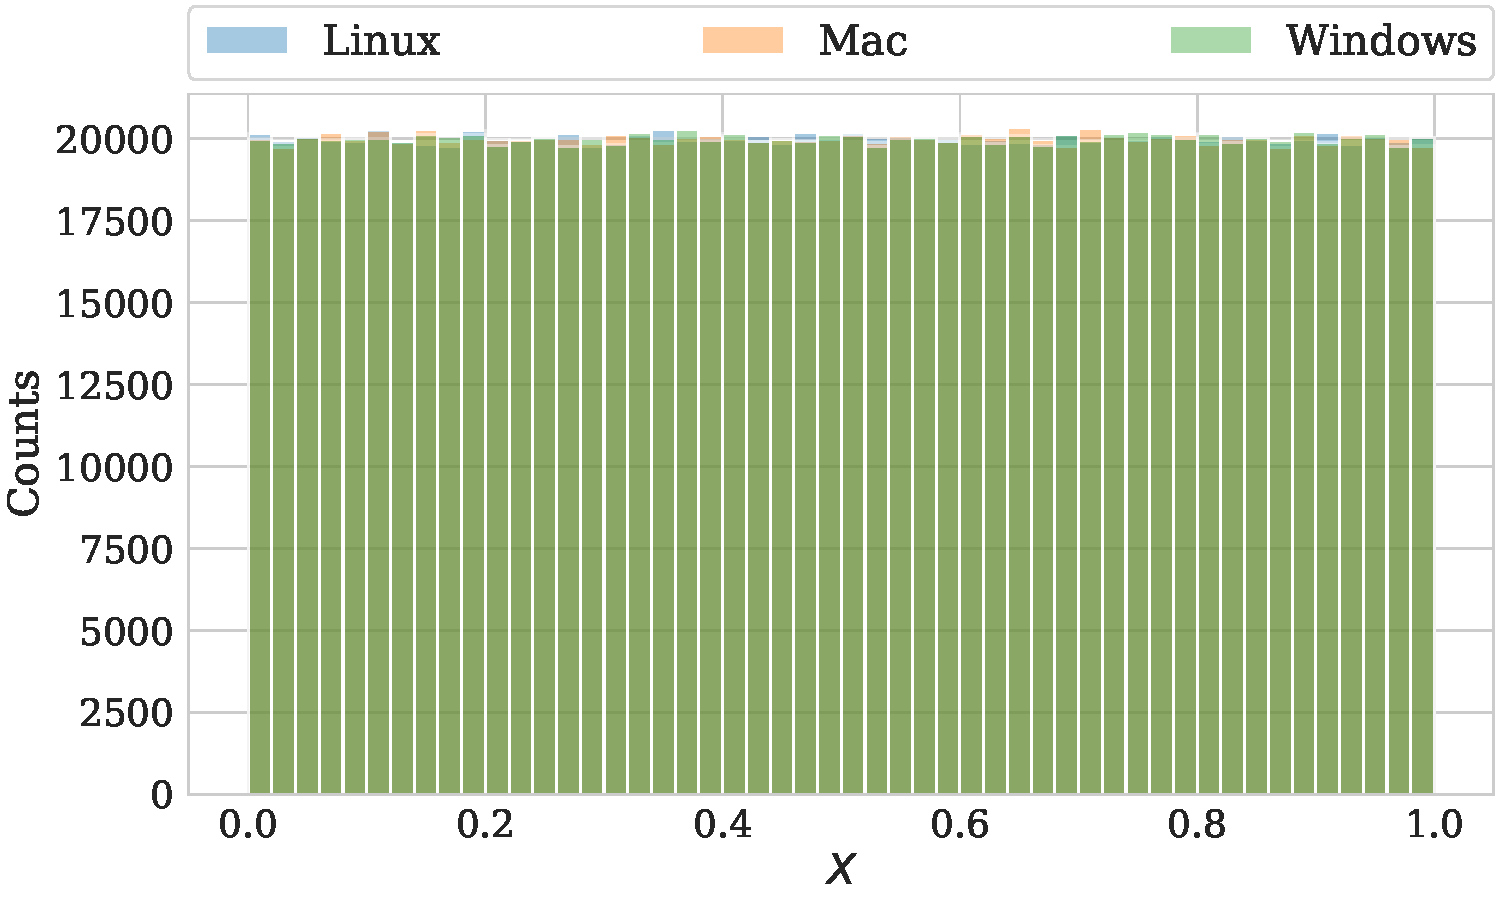
\includegraphics[width=\textwidth]{uniform}
      \caption{$X \sim \mathcal{N}(0.5, 0.2)$}
  \end{subfigure}
  \hfill
  \begin{subfigure}[b]{0.49\textwidth}
      \centering
      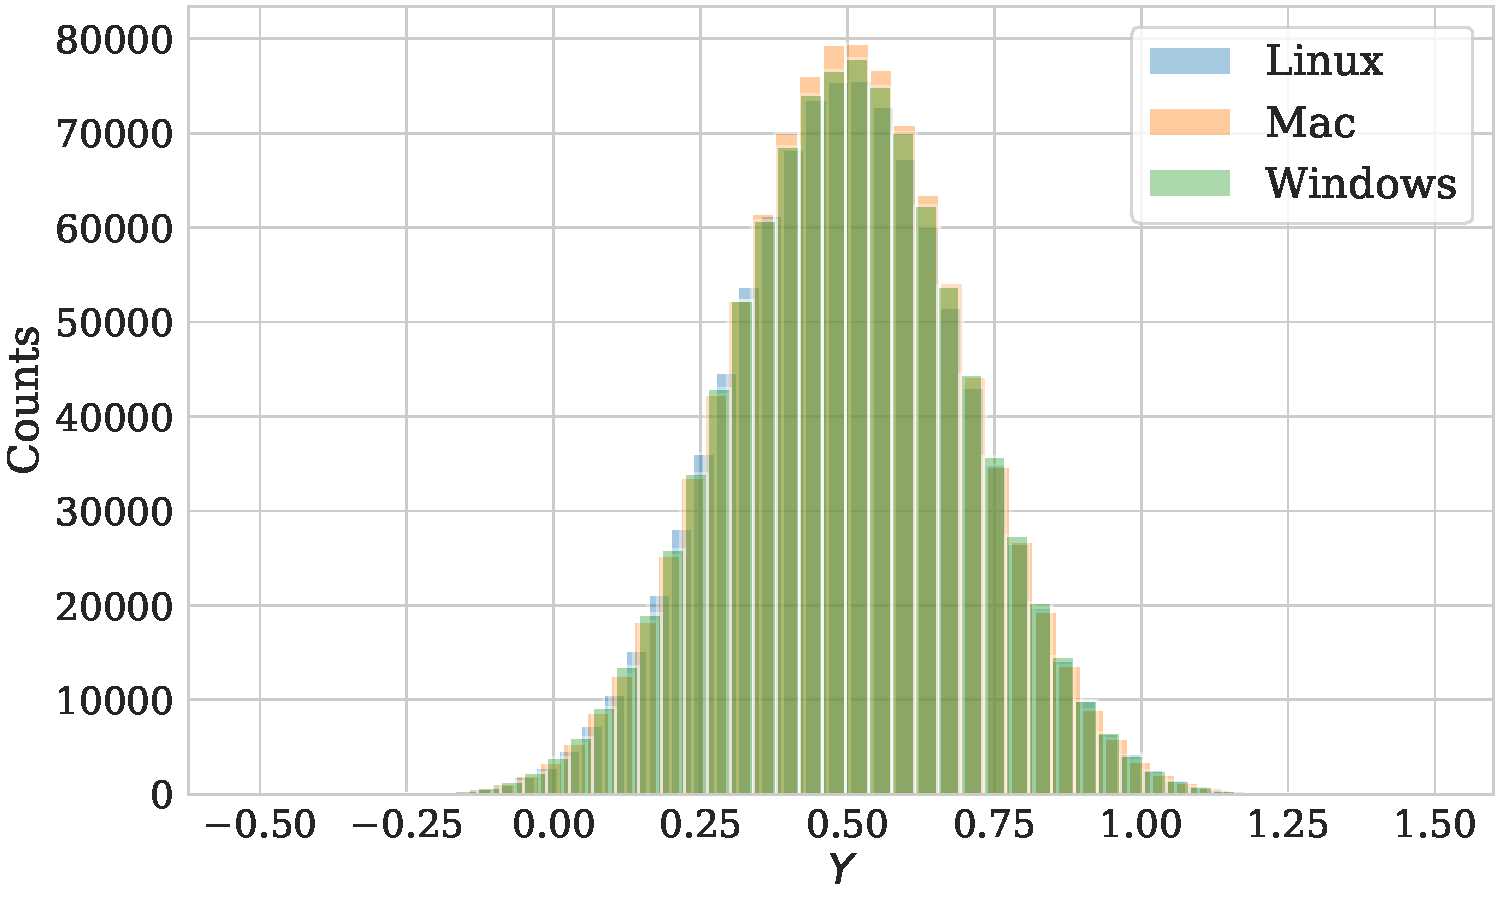
\includegraphics[width=\textwidth]{normal}
      \caption{$X \sim \mathcal{U}(0, 1)$}
  \end{subfigure}
    \caption{Histogram of used distributions}
    \label{fig:randomCheck}
\end{figure}

\subsection{Scheduler Cost Map}

\begin{figure}[htbp]
  \centering
  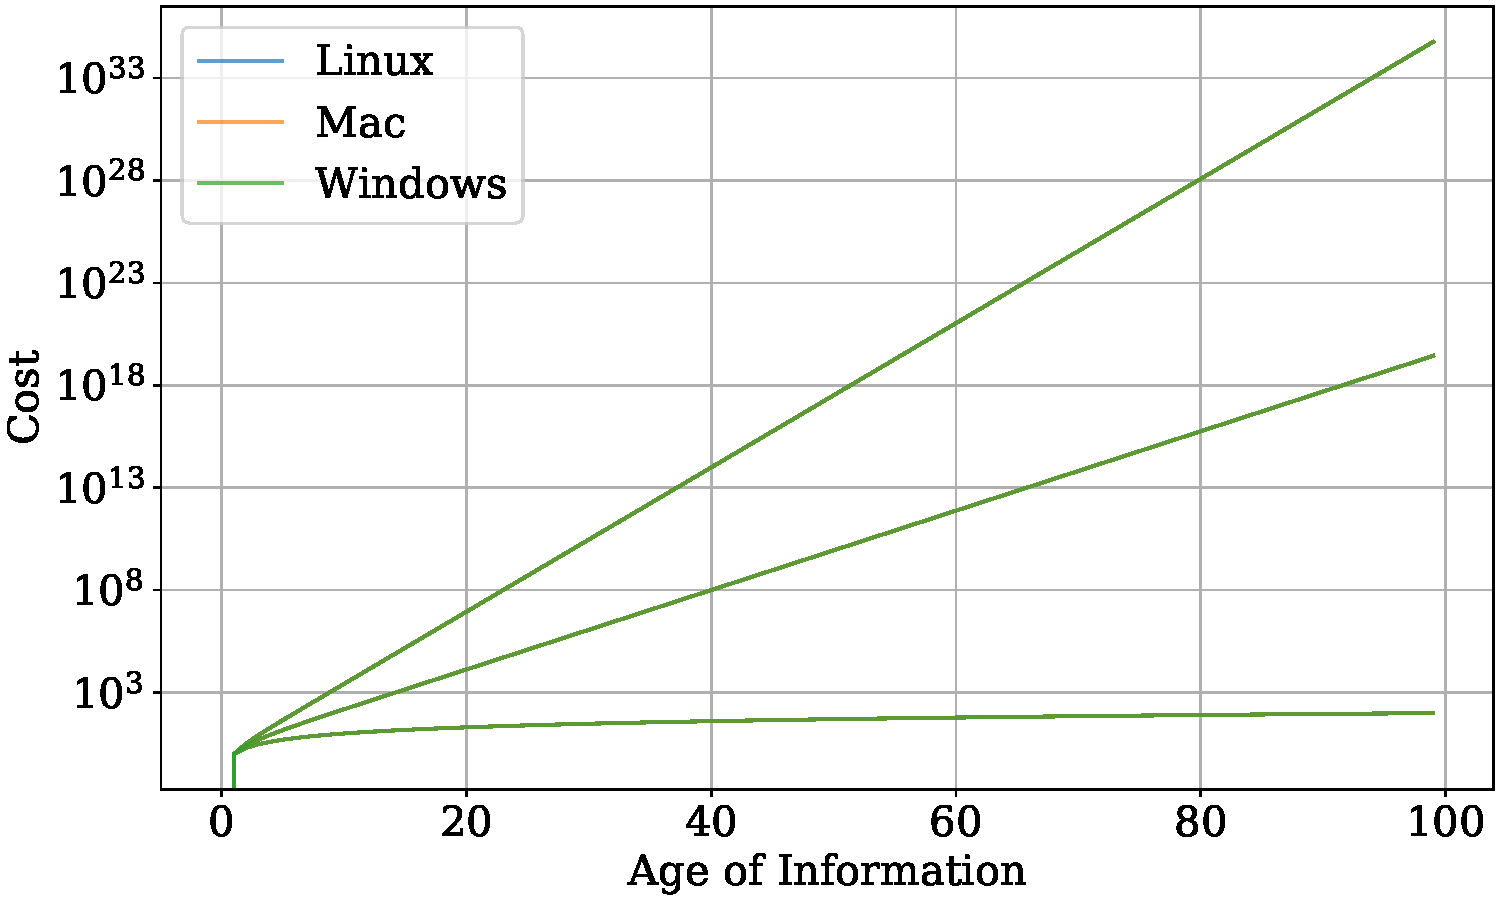
\includegraphics[width=0.8\textwidth]{costMaps} 
  \caption{Cost maps of scheduler}
  \label{fig:costmaps}
\end{figure}

\subsection{Discussion}
